%Dokumentinformationen
\newcommand{\titleinfo}{Analysis 2E - Formelsammlung}
\newcommand{\authorinfo}{F. Braun, L. Schmid, U. Giger, R. Koller, E. Ammann, S. Arnold, C. Gwerder, S. Koerner, L. Leuenberger}
\newcommand{\versioninfo}{$Revision: $ \today}

% standard header
%Schriftgr�sse, Layout, Papierformat, Art des Dokumentes
\documentclass[10pt,twoside,a4paper,fleqn]{article}
%Einstellungen der Seitenr�nder
\usepackage[left=1cm,right=1cm,top=1cm,bottom=1cm,includeheadfoot]{geometry}
% Sprache, Zeichensatz, packages
\usepackage[utf8]{inputenc}
\usepackage[ngerman]{babel,varioref}
\usepackage{amssymb,amsmath,fancybox,graphicx,color,lastpage,wrapfig,fancyhdr,hyperref,verbatim}

%pdf info
\hypersetup{pdfauthor={\authorinfo},pdftitle={\titleinfo},colorlinks=false}
%linkbordercolor=white
\author{\authorinfo}
\title{\titleinfo}

%Kopf- und Fusszeile
\pagestyle{fancy}
\fancyhf{}
%Linien oben und unten
\renewcommand{\headrulewidth}{0.5pt} 
\renewcommand{\footrulewidth}{0.5pt}

\fancyhead[L]{\titleinfo{ }\tiny{(\versioninfo)}}
%Kopfzeile rechts bzw. aussen
\fancyhead[R]{Seite \thepage { }von \pageref{LastPage}}
%Fusszeile links bzw. innen
\fancyfoot[L]{\footnotesize{\authorinfo}}
%Fusszeile rechts bzw. ausen
\fancyfoot[R]{\footnotesize{\today}} % ./header.tex nicht editieren (Projekt LaTeX-Header benutzen)

%%%%%%%%%%%%%%%%%%%%%%%%%%%%%%%%%%%%%%%%%%%%%%%%%%%%%%%%%%%%%%%%%%%%%%%%%%%%%%%%%%%%%%%%%%%%%%%%
% Neue Befehle und Definitionen                
%%%%%%%%%%%%%%%%%%%%%%%%%%%%%%%%%%%%%%%%%%%%%%%%%%%%%%%%%%%%%%%%%%%%%%%%%%%%%%%%%%%%%%%%%%%%%%%
\definecolor{black}{rgb}{0,0,0}
\definecolor{red}{rgb}{1,0,0}
\definecolor{white}{rgb}{1,1,1}
\definecolor{grey}{rgb}{0.8,0.8,0.8}
\newcommand{\formelbuch}[1]{$_{\textcolor{red}{\mbox{\small{S#1}}}}$}
\newcommand{\verweis}[2]{\small{(siehe auch \ref{#1}, #2 (S. \pageref{#1}))}}
\newcommand{\subsubadd}[1]{\textcolor{black}{\mbox{#1}}}

% This is needed for one more subsection, ex. 1.1.1.1, is called by \paragraph{}
\usepackage{titlesec}
\setcounter{secnumdepth}{4}
\setcounter{tocdepth}{4}
\titleformat{\paragraph}
{\normalfont\normalsize\bfseries}{\theparagraph}{1em}{}
\titlespacing*{\paragraph}
{0pt}{2.25ex plus 1ex minus .2ex}{1.0ex plus .2ex}

% This is needed for a smaller itemlist, is called by \compactenum {}
\usepackage{paralist}

% This is needed for merging some columns in a table
\usepackage{multicol} 
\usepackage{multirow} 

\begin{document}

\setlength{\parindent}{0pt}
           
%%%%%%%%%%%%%%%%%%%%%%%%%%%%%%%%%%%%%%%%%%%%%%%%%%%%%%%%%%%%%%%%%%%%%%%%%%%%%%%%%%%%%%%%%%%%%%%%
%%%%%%%%%%%%%%%%%%%%%%%%%%%%%%%%%%%%%%%%%%%%%%%%%%%%%%%%%%%%%%%%%%%%%%%%%%%%%%%%%%%%%%%%%%%%%%%%
\section{Integralrechnung \formelbuch{492}}
\subsection{Integrationsmethoden \formelbuch{495ff}}
\renewcommand{\arraystretch}{2}
\begin{tabular}{| l | l |}
	\hline
		Linearität &
			$\int{f(\alpha x+\beta )dx=\frac{1}{\alpha}\cdot F(\alpha x+\beta)+C}$ \\
	\hline
		Partielle Integration &
			$\int\limits_a^b{u'(x)\cdot v(x)dx}=\biggl[ u(x)\cdot v(x) \biggr]_a^b-\int\limits_a^b{u(x)\cdot v'(x)dx}$ \\
	\hline
		Weierstrass-Substitution &
			$t=\tan\frac{x}{2}, \qquad dx=\frac{2dt}{1+t^2}$
			$\qquad \sin  x=\frac{2t}{1+t^2}$
			$\qquad \cos x=\frac{1-t^2}{1+t^2} \quad\int{R(\sin(x),\cos(x))dx}$ \\
	\hline
		Allgemeine Substitution &
			$\int\limits_{a}^{b}{f(x)dx}=\int\limits_{g^{-1}(a)}^{g^{-1}(b)}{f(g(t))\cdot g'(t)dt}$
			$\qquad t=g^{-1}(x)$
			$\qquad  \fbox{x=g(t)}\Leftrightarrow^{d(...)} dx=g'(t)\cdot dt$ \\
	\hline
		Logarithmische Integration &
			$\int{\frac{f'(x)}{f(x)}dx}=\ln|f(x)|+C$
			$\qquad {(f(x)\neq 1)}$
			$\qquad y'(x)\cdot dx = dy \rightarrow$ allg. gültig\\
	\hline
		Potenzregel &
			$\int{f'(x)\cdot (f(x))^{\alpha} dx}=\frac{f(x)^{\alpha +1}}{\alpha+1}+C$
			$\qquad{(\alpha \neq -1)}$ \\
	\hline
		Differentiation &
			$\int \limits ^{b} _{a} {f'(t)dt}=f(b)-f(a)$
			$\qquad \frac{d}{dx} \int \limits ^{x} _{1} {f(t)dt}=f(x)$ \\
	\hline
			Mittelwerte &
				linear: $\frac{1}{b-a} \int\limits ^{b} _{a} {f(x)dx}$
				$\qquad$ quadratisch: $\sqrt{\frac{1}{b-a} \int\limits ^{b} _{a} {\lvert f(x)^2 \rvert dx}}$ \\
	\hline
\end{tabular}
\renewcommand{\arraystretch}{1}


\subsubsection{Einige unbestimmte Integrale \formelbuch{1081ff}} 
 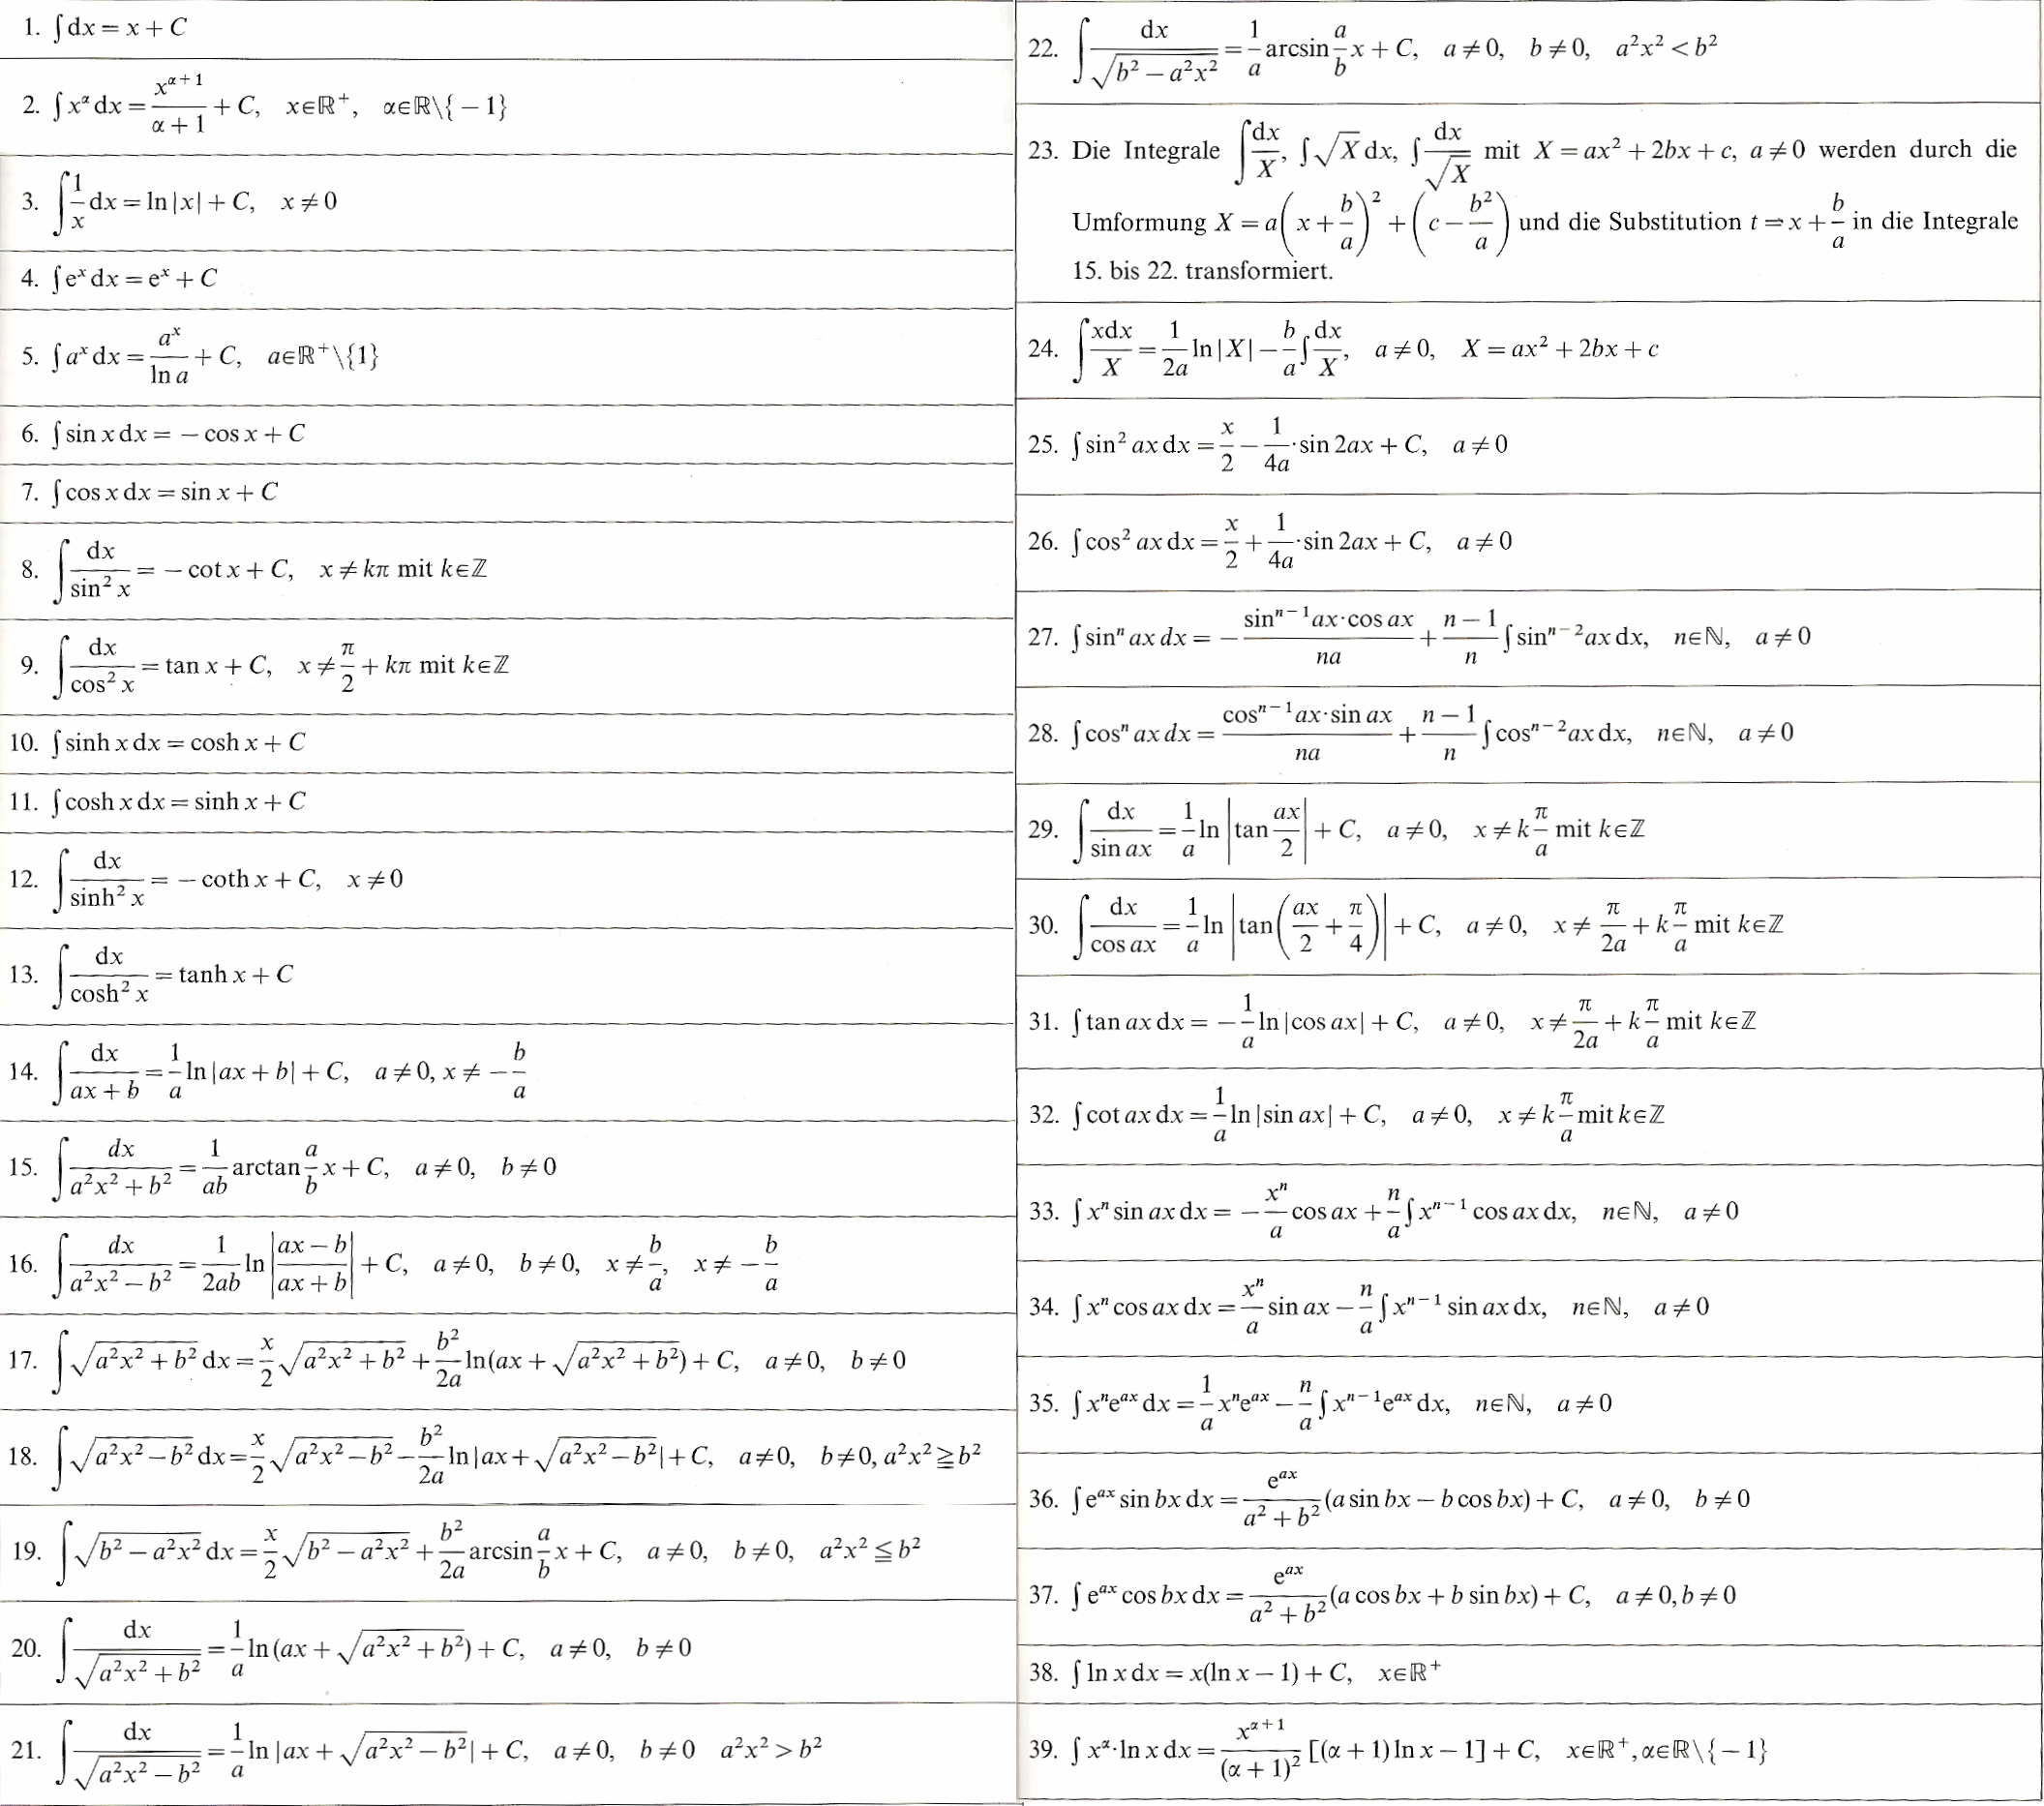
\includegraphics[width=16.1cm]{./bilder/integrale.png} 



\subsection{Uneigentliche Integrale\formelbuch{518}}
	Uneigentliches Integral heisst, dass entweder eine \textbf{unbeschränkte
	Funktion} integriert wird, oder eine Funktion über einen \textbf{unbeschränkten Integrationsberech} 
	integriert wird.$\\$
	\begin{minipage}{100mm}
    
	Für unbeschränkte Funktionen:$\\$
	$I =\int\limits _{a}^{c}f(x)dx=
	\lim\limits_{t\uparrow b}\int\limits_{a}^{t}f(x)dx+\lim\limits_{t\downarrow b}\int\limits_{t}^{c}f(x)dx\\
	\\$ Für die unbeschränkte Integration:$\\$
	$I =\int\limits _{a} ^{\infty} f(x)dx= \lim \limits_{t\to \infty}\int \limits
	_{a} ^{t}f(x)dx;\\$
	$I =\int\limits ^{a} _{-\infty} f(x)dx= \lim \limits_{t\to -\infty}\int
	\limits _{t} ^{a}f(x)dx; \\$
	$I =\int\limits _{-\infty} ^{\infty} f(x)dx = \lim \limits_{t_1\to -\infty} \lim
	\limits
	_{t_2 \to  \infty}\int \limits _{t_1} ^{a}f(x)dx + \int\limits_{a}^{t_2}f(x)dx\\$
	Beispiel: $\int\limits_{1}^{\infty}\frac{1}{x^2}dx=\lim\limits_{t\to \infty}\int\limits_{1}^{t}\frac{1}{x^2}dx=\lim\limits_{t\to \infty}-\frac{1}{t}+\frac{1}{1}=1$
    \end{minipage}
	\begin{minipage}{100mm}
    	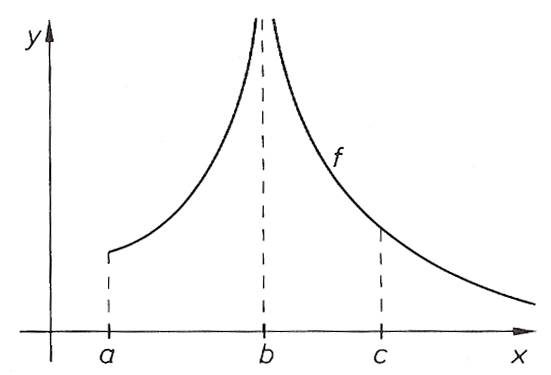
\includegraphics[width=3cm]{./bilder/unbeschraenkteFunktion.png} $\\$
    	unbeschränkte Funktion
    \end{minipage}

\subsubsection{Prinzip der Restfläche}
	Wenn $\lim\limits_{t \rightarrow \infty} \int\limits^{\infty}_{t} f(x) dx = 0$, dann konvergiert
	$\int\limits_a^{\infty} f(x) dx$ und umgekehrt.

\subsubsection{Majorantenprinzip}
	Um nachzuweisen, ob eine Funktion $|f(x)| \geq 0$ absolut konvergiert, wird eine zweite
	Funktion $g(x) \geq |f(x)|$ (Majorante) gesucht. Konvergiert $\int\limits_a^{\infty} g(x) dx$,
	dann konvergiert auch $\int\limits_a^{\infty} |f(x)| dx$ und somit konvergiert auch $\int\limits_a^{\infty} f(x) dx$. $\qquad x \in [a, \infty[$

\subsubsection{Minorantenprinzip}
	Um nachzuweisen, ob eine Funktion $f(x)$ divergiert, wird eine zweite
	Funktion $0 \leq g(x) \leq f(x)$ (Minorante) gesucht. Divergiert
	$\int\limits_a^{\infty} g(x) dx$,
	dann divergiert auch $\int\limits_a^{\infty} f(x) dx$. $\qquad x \in [a, \infty[$
	

%%%%%%%%%%%%%%%%%%%%%%%%%%%%%%%%%%%%%%%%%%%%%%%%%%%%%%%%%%%%%%%%%%%%%%%%%%%%%%%%%%%%%%%%%%%%%%%%
%%%%%%%%%%%%%%%%%%%%%%%%%%%%%%%%%%%%%%%%%%%%%%%%%%%%%%%%%%%%%%%%%%%%%%%%%%%%%%%%%%%%%%%%%%%%%%%%
%newpage
\section{Anwendung der Differential- und Integralrechnung}

\subsection{Beschreibungungsvarianten}
	\begin{minipage}[t]{3.5cm}
		Funktion (explizit) \\
		$ y = f(x)$ \\
        \tiny{(Bronstein S.49, 147)}
	\end{minipage}
	\begin{minipage}[t]{6cm} 		
		Koordinatengleichung (implizit) \\
		$ F(x,y) = 0 $ \\
        \tiny{(Bronstein S.49)}
	\end{minipage}
	\begin{minipage}[t]{5.5cm} 		
		Parameterform(Cartesisch) \\
		$ \left( \begin{array} {l} x(t) \\ y(t) \end{array} \right) =
          \left( \begin{array} {l} \Psi(t) \\ \varphi(t) \end{array} \right)$\\
        \tiny{(Bronstein S.49)}
	\end{minipage} 
	\begin{minipage}[t]{3cm}
    	Polarform x\\
    	$ r=f(\varphi) $ \\
    \end{minipage}\\

	$\rightarrow$ Ordnung immer ohne $\sqrt{\text{ }}$ \\

\subsection{Umrechnen diverser Systeme \formelbuch{49}}
\begin{tabular}{| l l | l|}
\hline Parameter 
	& $\Rightarrow$ explizit
	%& $x = f(t) \; \; y = g(t)$
	& $ t = f(x);\; y = g(f(x))$\\
\hline Explizit
	& $\Rightarrow$ Parameter
	%& $y = f(x)$
	& $ \left( \begin{array} {l} x(t) \\ y(t) \end{array} \right) =
          \left( \begin{array} {l} t \\ g(t) \end{array}
          \right)$ \\
\hline Ex- bzw. implizit 
	& $\Rightarrow$ Polar
	%& $y = f_1(x)$ bzw. $f_2(x,y) = C$
	&  Ersetze $x = r \cos(\varphi)$ ; $y = r \sin(\varphi)$ ; $x^2+y^2 = r^2$\\ 
\hline Polar 
	& $\Rightarrow$ implizit
	%& $r = f(\varphi)$
	& Ersetze $r \sin(\varphi) = y$; $r \cos(\varphi)=x$; $r=\sqrt{x^2 + y^2}$\\ 
\hline Polar
	& $\Rightarrow$ Parameterform
	%& $r = f(\varphi)$
	& $\left( \begin{array} {l} x(\varphi) \\ y(\varphi) \end{array} \right) =
          \left( \begin{array} {l} r(\varphi) \cos(\varphi) \\ r(\varphi) \sin(\varphi) \end{array}
          \right)$ \\
\hline Einzelner Punkt  
	& $\Rightarrow$ Polar
	%& $(x,\; y)$
	& $r = \sqrt{x^2 + y^2};\;
	\varphi = \begin{cases}\arctan(\frac{y}{x}) + \pi 	&x < 0\\
             \arctan(\frac{y}{x}) 	& x > 0\\
             \frac{\pi}{2}			& x = 0;\; y > 0\\
             -\frac{\pi}{2}			& x = 0;\; y < 0\\
             \text{unbestimmt}		& x = y = 0\end{cases}$\\
\hline
\end{tabular}

\subsection{Kurvenarten\formelbuch{203ff}}
$ \left.\begin{matrix}
	\text{bei `+`, Kurve auf linke Seite geöffnet}\\ 
	\text{bei `-`, Kurve auf rechte Seite geöffnet}
\end{matrix}\right\rbrace $ 
bei Polarform

\begin{tabular}{llll}
\parbox{2.7cm}{
\textbf{ } \\
Implizit:\\
Bemerkung:\\
Polarform:\\
Parameterform:\\
$p, \epsilon$:
}

\parbox{6cm}{
\textbf{Kreis\formelbuch{203}}\\
$(x-x_0)^2 + (y - y_0)^2 = r^2$\\
Mittelpunkt $(x_0, y_0)$; Radius $r$\\
$r = \frac{p}{1 + \epsilon \cos(\varphi)}; \epsilon = 0$\\
$x=x_0 + R\cos(t), y=y_0 + R\sin(t) $ \\
$ p = \frac{b^2}{a}$
} 

\parbox{8cm}{
\textbf{Ellipse\formelbuch{204}}\\
$(\frac{x-x_0}{a})^2 + (\frac{y-y_0}{b})^2 = 1$\\
Mittelpunkt $(x_0, y_0)$; Halbachsen $a$, $b$\\
$r = \frac{p}{1 + \epsilon \cos(\varphi)}; 0 < \epsilon < 1 \qquad$ (rechter Brennpunkt)\\
$x = a\cos(t), y = b\sin(t) \qquad$ um $P(0,0)$ \\
$\epsilon = \frac{c}{a}$
}\\ \\


\parbox{2.7cm}{
\textbf {}\\
Implizit:\\
Bemerkung:\\
Polarform:\\
Parameterform:
}

\parbox{6cm}{
\textbf{Hyperbel\formelbuch{206}}\\ 
$(\frac{x}{a})^2 - (\frac{y}{b})^2 = 1; -(\frac{x}{a})^2 + (\frac{y}{b})^2 =1$\\ 
Achsenkreuz in $P(0,0)$\\
$r = \frac{p}{1 - \epsilon \cos(\varphi)}; \epsilon > 1_{(rechter Hyperbelast)}$\\
$r = \frac{p}{1 + \epsilon \cos(\varphi)}_{(linker Hyperbelast)}$ \\
$x= a \cosh(t), y = b \sinh(t) $ 

}

\parbox{8cm}{
\textbf{Parabel\formelbuch{209}}\\
$y^2 = 2p(x-x_0)$\\
Parabeln mit Scheitelpunkt auf der vertikaler Achse\\
$r = \frac{p}{1 - \epsilon \cos(\varphi)}; \epsilon = 1$\\
$x= \frac{t^2}{2p}, y = t$\\
$p=$Halbparameter (2$\cdot$Abstand Scheitel-Brennpunkt)
}\\ \\

\parbox{2.7cm}{
\textbf{} \\
Polarform:
}

\parbox{5cm}{
\textbf{Kardioide/Herzk. \formelbuch{99}} \\
$r = a(1+\cos(\varphi))$
}

\parbox{5cm}{
\textbf{Lemniskate ``$\infty$'' \formelbuch{101}} \\
$r = a\sqrt{2\cos(2\varphi)}$ 
}

\parbox{5cm}{
\textbf{Strophoide/harm. K. \formelbuch{96}} \\
$ r = -a \frac{\cos(2\varphi)}{\cos(\varphi)},(a>0) $ 
}

\end{tabular}

\subsection{Gleichungen, Mittelwerte\formelbuch{19ff, 509}}
\begin{tabular}{llll}
	\textbf{Tangentengleichung} &
	\textbf{Normalengleichung} &
	\textbf{Linearer Mittelwert} &
	\textbf{Quadratischer Mittelwert}\\
	$y-y_0=f'(x_0)(x-x_0)$ &
	$y-y_0=-\frac{1}{f'(x_0)}(x-x_0)$ &
	$\bar{f} = \frac{1}{b-a} \int\limits_{a}^{b} f(x)dx$ &
	$\bar{f} = \sqrt{\frac{1}{b-a} \int\limits_{a}^{b} f(x)^2dx}$ \\
	$\dot{x_0}(y-y_0) = \dot{y_0}(x-x_0)$ \\
\end{tabular}
	
\subsection{Tangenten- \& Normalenabschnitt, Subtangente \& Subnormale\formelbuch{251ff}}

\subsection{Abstandsformeln}
\begin{tabular}{p{7cm}p{5cm}p{6cm}l}
	\textbf{Hessesche Normalform\formelbuch{200f, 224}} &
	\textbf{Geradengleichung} &
	\textbf{Abstand zum Ursprung} \\
	$x\cdot \cos\varphi_0 +y\cdot \sin\varphi_0=r_0$ &
	$y - y_0 = m (x - x_0)$ &
	$\frac{|y_0 - m \cdot x_0|}{\sqrt{m^2 + 1}}$ \\
	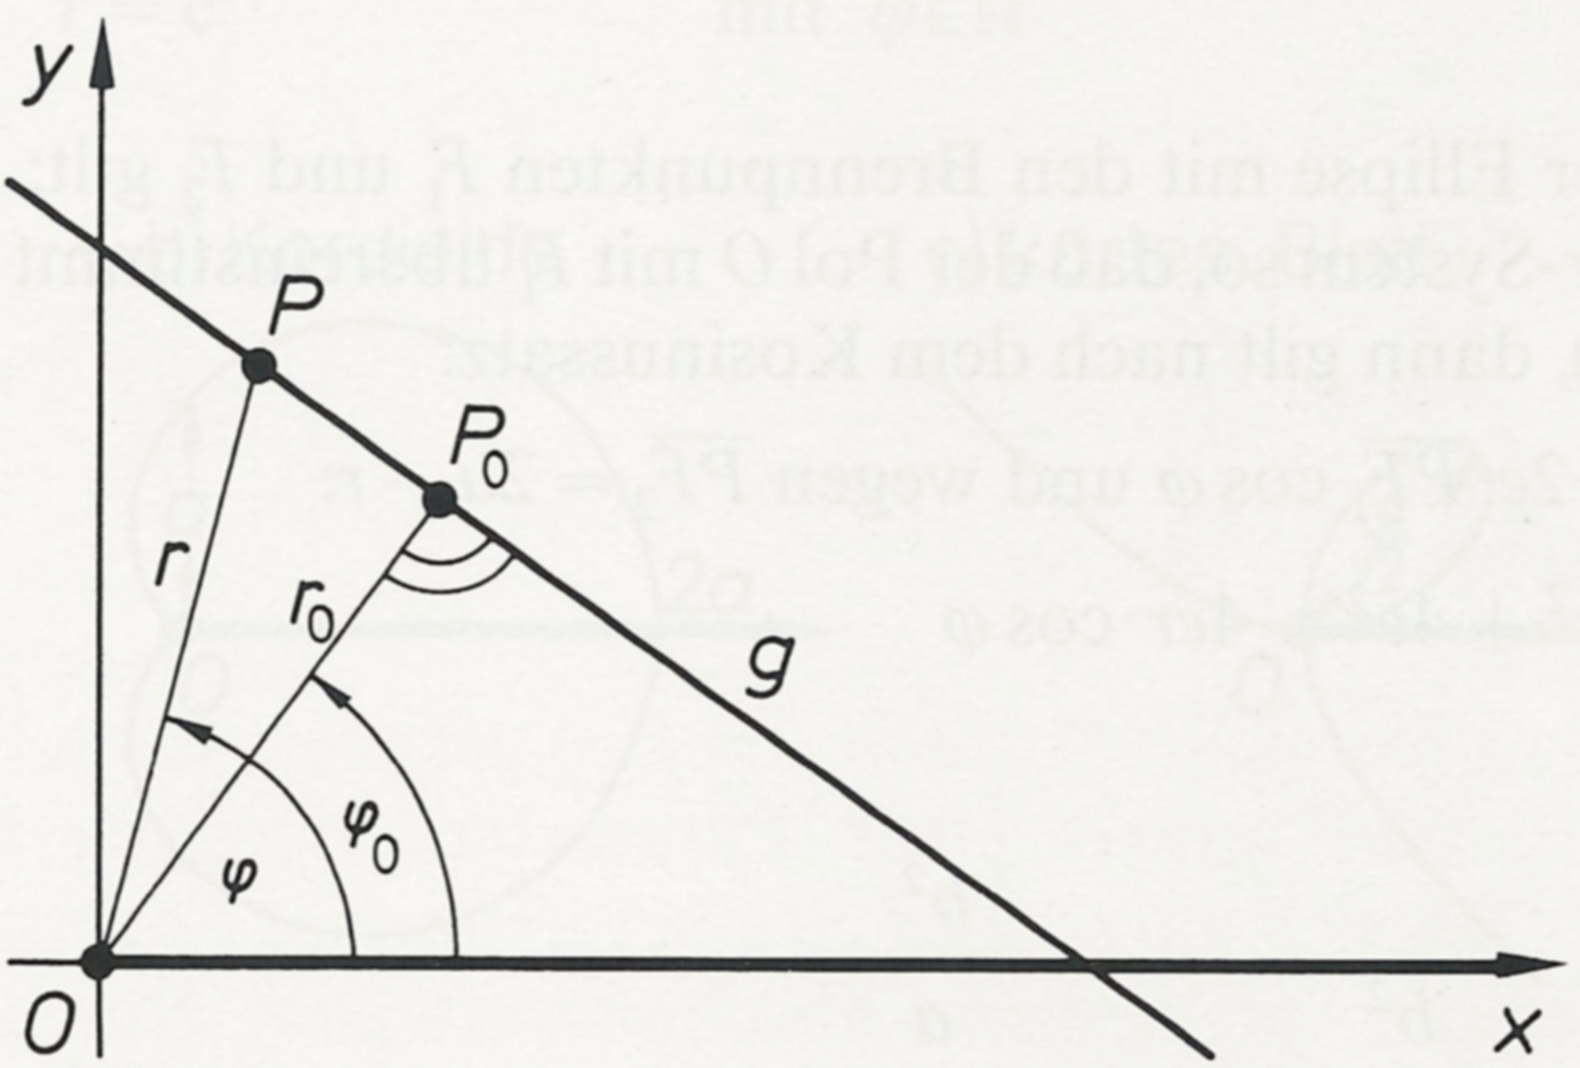
\includegraphics[width=6cm]{./bilder/hessenorm.png} \\
\end{tabular}


\subsection{Berührung in n-ter Ordnung}
Zwei explizit gegebene Kurven $y = f(x)$ und $y = g(x)$ berühren einander im
Punkt P $x_0, y_0$ von der Ordnung $n$, wenn die Funktionswerte und die ersten
$n$ Ableitungen existieren und übereinstimmen.\\
$f(x_0) = g(x_0);\; f'(x_0) = g'(x_0);\; f''(x_0) = g''(x_0);\;\ldots ;
\;f^{(n)}(x_0) = g^{(n)}(x_0)\; \qquad f^{(n+1)}(x_0) \neq g^{(n+1)}(x_0)$

\subsection{Scheitel \formelbuch{256}}
Scheitelpunte sind Extremalwerte der Krümmungs- bzw. Krümmungsradiusfunktion.
Falls bei $\kappa'(x)$ an der Stelle $x_0$ ein Vorzeichenwechsel besteht, existiert dort
eine Extremalstelle. 
$\qquad \kappa'(x) = 0; \kappa''(x) \neq 0$

\subsection{Wichtige Formeln\formelbuch{249ff}}
	\renewcommand{\arraystretch}{2}
	\begin{tabular}[c]{ | p{5.1cm} | p{5.4cm} | l | }
		\hline
		\textbf{Cartesisch} & \textbf{Parameter} & \textbf{Polar} \\
		\hline
		\multicolumn{3}{| l |}{\textbf{Anstieg einer Kurve, Ableitung, 2. Ableitung}} \\
    	\hline   
    	$y'=f'(x_o) \quad y'' = f''(x_0)$ & 
    	$y'=\frac{\dot{y}}{\dot{x}} \quad 
    	y'' = \frac{\dot{x} \ddot{y} - \dot{y}\ddot{x}}{\dot{x}^3}$ &
    	$y'=\frac{r'(\varphi) \sin(\varphi) + r(\varphi) \cdot
    	\cos(\varphi)}{r'(\varphi) \cos(\varphi)-r(\varphi) \cdot \sin(\varphi)}$
    	\\
		
		\hline
		\multicolumn{3}{| l |}{\textbf{Bogenlänge \formelbuch{514}}} \\
    	\hline
    	$s=\int\limits_a^b{\sqrt{1+(f'(x))^2}dx}$ & 
    	$|s|=\int\limits_{t_1}^{t_2}{\sqrt{\dot{x}^2(t)+\dot{y}^2(t)}dt}$ &
		$|s|=\int\limits_{\varphi_1}^{\varphi_2}{\sqrt{(r'(\varphi))^2+(r(\varphi))^2}d\varphi}$\\
		
		\hline		
		\multicolumn{3}{| l |}{\textbf{Krümmung ebener Kurven \formelbuch{253}}}\\
    	\hline
    	$\kappa=\frac{f''(x)}{(\sqrt{1+(f'(x))^2})^3}$ &
    	$\kappa=\frac{\dot{x}(t)\ddot{y}(t)-\dot{y}(t)\ddot{x}(t)}{(\sqrt{(\dot{x}(t))^2+(\dot{y}(t))^2})^3}$ &
		$\kappa=\frac{2(r'(\varphi))^2-r(\varphi)r''(\varphi)+(r(\varphi))^2}{(\sqrt{(r'(\varphi))^2+(r(\varphi))^2})^3}$\\   	
		
		\hline
		\multicolumn{3}{| l |}{Konvex (Linkskurve): $\kappa \geq 0 \qquad$ Streng
		konvex: $\kappa > 0 \qquad$ Wendepunkt: $\kappa = 0 \qquad$ Analog für konkav}\\
		
		\hline
		\multicolumn{3}{| l |}{\textbf{Krümmungskreisradius \formelbuch{253}} $\qquad r = |\frac{1}{\kappa}|$} \\
		\hline
		$r = \left|\frac{(\sqrt{1+(f'(x))^2})^3}{f''(x)} \right|$ &
		$r = \left|\frac{(\sqrt{(\dot{x}(t))^2+(\dot{y}(t))^2})^3}
		{\dot{x}(t)\ddot{y}(t)-\dot{y}(t)\ddot{x}(t)} \right|$ & 
		$r = \left|\frac{(\sqrt{(r'(\varphi))^2+(r(\varphi))^2})^3}
		{2(r'(\varphi))^2-r(\varphi)r''(\varphi)+(r(\varphi))^2} \right|$ \\
		
		\hline		
		\multicolumn{3}{| l |}{\textbf{Flächeninhalt \formelbuch{513}} um x-Achse /  für y-Achse: $f(y)$ von $y_0$ bis $y_1$ integrieren} \\
    	\hline
    	$A=\int\limits_a^b{f(x)}dx$  & 
    	$A=\frac{1}{2}\int\limits_{t_1}^{t_2}{[x(t)\dot{y}(t)-\dot{x}(t)y(t)]dt}$ &
		$A=\frac{1}{2}\int\limits_{\varphi_1}^{\varphi_2}{(r(\varphi))^2d\varphi}$\\  
    	
		\hline		
		\multicolumn{3}{| l |}{\textbf{Volumen \formelbuch{514}} um x-Achse 
		 / für y-Achse: $f(y)$ von $y_0$ bis $y_1$ integrieren
		 / Nur 1.Hälfte der Kurve integrieren!} \\
    	\hline
		$V=\pi\int\limits_a^b(f(x))^2dx$ & 
    	$V=\pi\left|\int\limits_{t_1}^{t_2}{(y(t))^2\dot{x}(t)dt}\right|$ &
		$V=\pi\left|\int\limits_{\varphi_1}^{\varphi_2}{r^2(\varphi)\sin^2\varphi[r'(\varphi)\cos(\varphi)-r(\varphi)\sin(\varphi)]d\varphi}\right|$\\  
    	
		\hline		
		\multicolumn{3}{| l |}{\textbf{Oberflächeninhalt \formelbuch{514}} um x-Achse 
		 / für y-Achse: $f(y)$ von $y_0$ bis $y_1$ integrieren
		 / Nur 1.Hälfte der Kurve integrieren!} \\
    	\hline
   		$O=2\pi\int\limits_a^b{|f(x)|\sqrt{1+(f'(x))^2}dx}$ & 
    	$O=2\pi\int\limits_{t_1}^{t_2}{|y(t)|\sqrt{\dot{x}^2(t)+(\dot{y}^2(t))}dt}$ &
		$O=2\pi\int\limits_{\varphi_1}^{\varphi_2}{|r(\varphi)\sin\varphi|\sqrt{(r'(\varphi))^2+(r(\varphi))^2}d\varphi}$\\  
    	\hline
		\multicolumn{3}{| l |}{Polar: \qquad $\sin \varphi =$ Drehung um Polgerade \qquad $\cos y =$ Drehung um y-Achse $(f = \frac{\pi}{2}) \qquad \rightarrow$ siehe Fläche} \\
	\hline
		\multicolumn{3}{| l |}{\textbf{Krümmungskreismittelpunkt}} \\
	\hline
		$x_c = x - \frac{\frac{dy}{dx}[1 + (\frac{dy}{dx})^2]}{\frac{d^2y}{dx^2}}$&
		$ x_c = x - \frac{\dot{y}(\dot{x}^2 + \dot{y}^2)}{\dot{x}\ddot{y} - \ddot{x}\dot{y}} $ &
		$x_c = r\cdot \cos\varphi - \frac{(r^2 + r'^2)(r\cdot \cos\varphi + r' \cdot \sin\varphi)}{r^2 + 2r'^2 - r\cdot r''}$\\

		$y_c = y + \frac{1+ (\frac{dy}{dx})^2}{\frac{d^2y}{dx^2}}$&
		$y_c = y + \frac{\dot{x}(\dot{x}^2 + \dot{y}^2)}{\dot{x}\ddot{y} - \ddot{x}\dot{y}} $ &
		$y_c = r\cdot \sin\varphi - \frac{(r^2 + r'^2)(r\cdot \sin\varphi - r' \cdot \cos\varphi)}{r^2 + 2r'^2 - r\cdot r''}$\\
	\hline
	\end{tabular}
	\renewcommand{\arraystretch}{1}
	
\subsection{Evolute}
Evolute = $\Sigma$ Krümmungskreiszentren\\
$\left(\begin{matrix} x_c \\ y_c \end{matrix}\right) = \left(\begin{matrix} x \\  y \end{matrix}\right) + \frac{1}{\kappa}\overrightarrow{n}$

\subsection{Orthogonaltrajektorien}
\begin{tabular}{ll}
\parbox{2.5cm}{
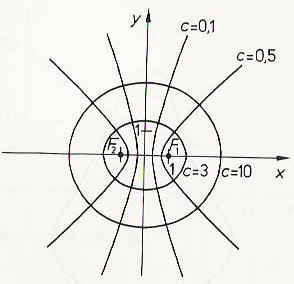
\includegraphics[height=2.5cm]{./bilder/orthoTrajekt.png}
}
& \parbox{16.5cm}{
Die orthogonalen Trajektorien schneiden alle Kurven der gegebenen Kurvenschar
$y=f(x,c)$ (c bestimmen) im rechten Winkel.
Die DGL $F(x,y,y')$ der Kurve bestimmen($y'$ ableiten, c einsetzen, wenn möglich für $f(x,c) = y$), anschliessend $y'$ durch
$-\frac{1}{y'}$ ersetzen.
$\Rightarrow$ ergibt die DGL der orthogonalen Trajektorien.\\
Die Kreise sind Orthogonaltrajektorien der Hyperbeln und umgekehrt.\\
$\frac{r'}{r} = f(\varphi , r) \qquad \underrightarrow{orthogonal}  \qquad \frac{r'}{r} = - \frac{1}{f(\varphi , r)}$
}
\end{tabular}

%%%%%%%%%%%%%%%%%%%%%%%%%%%%%%%%%%%%%%%%%%%%%%%%%%%%%%%%%%%%%%%%%%%%%%%%%%%%%%%%%%%%%%%%%%%%%%%%
%%%%%%%%%%%%%%%%%%%%%%%%%%%%%%%%%%%%%%%%%%%%%%%%%%%%%%%%%%%%%%%%%%%%%%%%%%%%%%%%%%%%%%%%%%%%%%%%

%newpage
\input{sections/Reihen.tex}
\newpage
\input{sections/Differentialgleichungen.tex}
\newpage

\section{Formeln + Theorie aus An1E}

%%%%%%%%%%%%%%%%%%%%%%%%%%%%%%%%%%%%%%%%%%%%%%%%%%%%%%%%%%%%%%%%%%%%%%%%%%%%%%%%%%%%%%%%%%%%%%%%
% Trigonometrie
%%%%%%%%%%%%%%%%%%%%%%%%%%%%%%%%%%%%%%%%%%%%%%%%%%%%%%%%%%%%%%%%%%%%%%%%%%%%%%%%%%%%%%%%%%%%%%%%	
\subsection{Trigonometrie}
	$\sin^2(b)+\cos^2(b)=1 \qquad \tan(b)=\frac{\sin(b)}{\cos(b)}$
	
\subsubsection{Funktionswerte für Winkelargumente}
	\renewcommand{\arraystretch}{1.5}
	\begin{minipage}{5cm}
		\begin{tabular}[c]{ |c|c||c|c|c| }
	    	\hline
			deg & rad & sin & cos & tan\\
			\hline
			0\symbol{23} & 0 & 0 & 1 & 0\\
			\hline
			30\symbol{23} & $\frac{\pi}{6}$ & $\frac{1}{2}$ & $\frac{\sqrt{3}}{2}$ &
			$\frac{\sqrt{3}}{3}$\\
			\hline
			45\symbol{23} & $\frac{\pi}{4}$ & $\frac{\sqrt{2}}{2}$ & $\frac{\sqrt{2}}{2}$
			& 1\\
			\hline
			60\symbol{23} & $\frac{\pi}{3}$ & $\frac{\sqrt{3}}{2}$ & $\frac{1}{2}$ &
			$\sqrt{3}$\\
			\hline			
		\end{tabular}			
	\end{minipage}
	\begin{minipage}{4.3cm}
		\begin{tabular}[c]{ |c|c||c|c|}
	    	\hline
			deg & rad & sin & cos\\
			\hline
			90\symbol{23} & $\frac{\pi}{2}$ & 1 & 0\\
			\hline	
			120\symbol{23} & $\frac{2\pi}{3}$ & $\frac{\sqrt{3}}{2}$ & $-\frac{1}{2}$ \\
			\hline
			135\symbol{23} & $\frac{3\pi}{4}$ & $\frac{\sqrt{2}}{2}$ & $-\frac{\sqrt{2}}{2}$\\
			\hline
			150\symbol{23} & $\frac{5\pi}{6}$ & $\frac{1}{2}$ & $-\frac{\sqrt{3}}{2}$\\
			\hline
		\end{tabular}			
	\end{minipage}
	\begin{minipage}{4.5cm}
		\begin{tabular}[c]{ |c|c||c|c| }
	    	\hline
			deg & rad & sin & cos\\
			\hline
			180\symbol{23} & $\pi$ & 0 & -1\\
			\hline	
			210\symbol{23} & $\frac{7\pi}{6}$ & $-\frac{1}{2}$ & $-\frac{\sqrt{3}}{2}$\\
			\hline
			225\symbol{23} & $\frac{5\pi}{4}$ & $-\frac{\sqrt{2}}{2}$ & $-\frac{\sqrt{2}}{2}$\\
			\hline
			240\symbol{23} & $\frac{4\pi}{3}$ & $-\frac{\sqrt{3}}{2}$ & $-\frac{1}{2}$\\
			\hline
		\end{tabular}			
	\end{minipage}
	\begin{minipage}{4.5cm}
		\begin{tabular}[c]{ |c|c||c|c| }
	    	\hline
			deg & rad & sin & cos\\
			\hline
			270\symbol{23} & $\frac{3\pi}{2}$ & -1 & 0\\
			\hline	
			300\symbol{23} & $\frac{5\pi}{3}$ & $-\frac{\sqrt{3}}{2}$ & $\frac{1}{2}$\\
			\hline
			315\symbol{23} & $\frac{7\pi}{4}$ & $-\frac{\sqrt{2}}{2}$ & $\frac{\sqrt{2}}{2}$\\
			\hline
			330\symbol{23} & $\frac{11\pi}{6}$ & $-\frac{1}{2}$ & $\frac{\sqrt{3}}{2}$\\
			\hline
		\end{tabular}			
	\end{minipage}
	\renewcommand{\arraystretch}{1}
	
\subsubsection{Periodizität}
	$\cos(a+k\cdot2\pi)=\cos(a) \qquad \sin(a+k\cdot2\pi)=\sin(a) \qquad
	(k \in \mathbb{Z})$
	
\subsubsection{Quadrantenbeziehungen}
	\begin{tabbing}
    	xxxxxxxxxxxxxxxxxxxxxxxxxxxxxxxxxx \= \kill
	 	$\sin(-a)=-\sin(a)$ \> $\cos(-a)=\cos(a)$\\
		$\sin(\pi - a)=\sin(a)$ \> $\cos(\pi - a)=-\cos(a)$\\
		$\sin(\pi + a)=-\sin(a)$ \> $\cos(\pi +a)=-\cos(a)$\\
		$\sin\left(\frac{\pi}{2}-a \right)=\sin\left(\frac{\pi}{2}+a \right)=\cos(a)$ \>
		$\cos\left(\frac{\pi}{2}-a \right)=-\cos\left(\frac{\pi}{2}+a \right)=\sin(a)$  
    \end{tabbing}

\subsubsection{Additionstheoreme}
		$\sin(a \pm b)=\sin(a) \cdot \cos(b) \pm \cos(a) \cdot \sin(b)$\\
		$\cos(a \pm b)=\cos(a) \cdot \cos(b) \mp \sin(a) \cdot \sin(b)$\\	
		$\tan(a \pm b)=\dfrac{\tan(a) \pm \tan(b)}{1 \mp \tan(a) \cdot \tan(b)}$

\subsubsection{Doppel- und Halbwinkel}	
		$\sin(2a)=2\sin(a)\cos(a)$\\
		$\cos(2a)=\cos^2(a)-\sin^2(a)=2\cos^2(a)-1=1-2\sin^2(a)$\\
		$\cos^2 \left(\frac{a}{2}\right)=\frac{1+\cos(a)}{2} \qquad
		\sin^2 \left(\dfrac{a}{2}\right)=\frac{1-\cos(a)}{2}$
		
\subsubsection{Produkte}
		$\sin(a)\sin(b)=\frac{1}{2}(\cos(a-b)-\cos(a+b))$\\
		$\cos(a)\cos(b)=\frac{1}{2}(\cos(a-b)+\cos(a+b))$\\
		$\sin(a)\cos(b)=\frac{1}{2}(\sin(a-b)+\sin(a+b))$
		
\subsubsection{Summe und Differenz}
		$\sin(a)+\sin(b)=2 \cdot \sin \left(\frac{a+b}{2}\right) \cdot
		\cos\left(\frac{a-b}{2}\right)$\\
		$\sin(a)-\sin(b)=2 \cdot \sin \left(\frac{a-b}{2}\right) \cdot
		\cos\left(\frac{a+b}{2}\right)$\\
		$\cos(a)+\cos(b)=2 \cdot \cos \left(\frac{a+b}{2}\right) \cdot
		\cos\left(\frac{a-b}{2}\right)$\\
		$\cos(a)-\cos(b)=-2 \cdot \sin \left(\frac{a+b}{2}\right) \cdot
		\cos\left(\frac{a-b}{2}\right)$\\
		$\tan(a) \pm \tan(b)=\dfrac{\sin(a \pm b)}{\cos(a)\cos(b)}$		
	




\end{document}
